\documentclass[border=4pt]{standalone}
\usepackage{tikz}
\usetikzlibrary{arrows}
\begin{document}
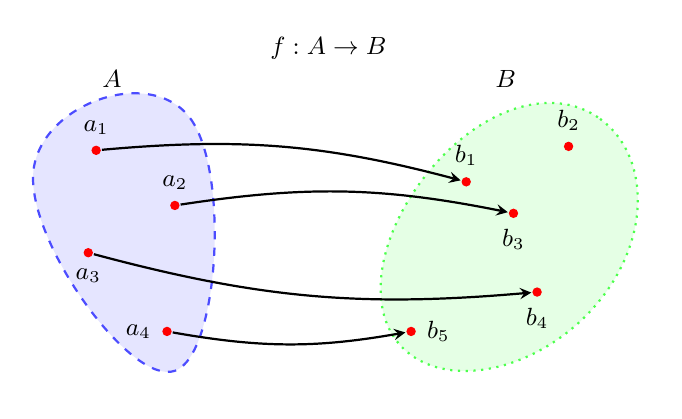
\begin{tikzpicture}[>=stealth, thick, font=\small]

    %%% Set A
    \begin{scope}
        % Draw a "freeform" shape for set A
        \draw[fill=blue!10, draw=blue!70, thick, dashed]
             plot[smooth cycle, tension=1] coordinates {
                (0,0) (2,0.7) (1.8,-2.5)
             };
        % Label A
        \node at (1,1.2) {$A$};

        % Points in A
        \node (a1) [circle, fill=red, inner sep=1.2pt, label=above:$a_{1}$] at (0.8,0.3) {};
        \node (a2) [circle, fill=red, inner sep=1.2pt, label=above:$a_{2}$] at (1.8,-0.4) {};
        \node (a3) [circle, fill=red, inner sep=1.2pt, label=below:$a_{3}$] at (0.7,-1.0) {};
        \node (a4) [circle, fill=red, inner sep=1.2pt, label=left:$a_{4}$]  at (1.7,-2) {};
    \end{scope}

    %%% Set B (shifted to the right)
    \begin{scope}[xshift=5cm]
        % Draw a "freeform" shape for set B
        \draw[fill=green!10, draw=green!70, thick, dotted]
             plot[smooth cycle, tension=1] coordinates {
                (0,0) (2.2,0.7) (2.2,-1.6) (-0.2,-2.3)
             };
        % Label B
        \node at (1,1.2) {$B$};

        % Points in B
        \node (b1) [circle, fill=red, inner sep=1.2pt, label=above:$b_{1}$] at (0.5,-0.1) {};
        \node (b2) [circle, fill=red, inner sep=1.2pt, label=above:$b_{2}$] at (1.8,0.35) {};
        \node (b3) [circle, fill=red, inner sep=1.2pt, label=below:$b_{3}$] at (1.1,-0.5) {};
        \node (b4) [circle, fill=red, inner sep=1.2pt, label=below:$b_{4}$] at (1.4,-1.5) {};
        \node (b5) [circle, fill=red, inner sep=1.2pt, label=right:$b_{5}$] at (-0.2,-2.0) {};
    \end{scope}

    %%% Label the function at the top
    \node at (3.75,1.6) {$f: A \to B$};

    %%% Draw arrows (the function)
    \draw[->] (a1) to[bend left=10]  (b1);
    \draw[->] (a2) to[bend left=10]  (b3);
    \draw[->] (a3) to[bend right=10] (b4);
    \draw[->] (a4) to[bend right=10] (b5);

\end{tikzpicture}
\end{document}
